\section{实验十:Mmap}\label{sec:Mmap}

\texttt{mmap} 和 \texttt{munmap} 系统调用允许 \texttt{UNIX} 程序对其地址空间进行精细控制。它们可用于在进程之间共享内存、将文件映射到进程地址空间,以及作为用户级页面错误方案(例如讲座中讨论的垃圾收集算法)的一部分。本实验将添加 \texttt{mmap} 和 \texttt{munmap} 到 xv6,重点关注内存映射文件。

\subsection{实验目的}

\begin{enumerate}
	\item 了解使用虚拟内存的原因和好处。 
    \item 理解创建和释放文件映射的方式。 
	\item 梳理文件内存映射的生命周期。 
\end{enumerate}

\subsection{实验内容}

添加 mmap 与 mumap 两个系统调用。前者将一个文件内存映射到进程的地址空间,后者取消已有地址空间的映射。

\subsection{实验准备}

\subsubsection{mmap}

将一个文件或者其他对象映射到进程的地址空间,实现文件磁盘地址和进程虚拟地址空间中一段虚拟地址的一一对应关系。

使用 mmap 的好处在于,常规的文件系统操作是用户态发起 read 系统调用,然后在 buffer cache 中查找是否有相应的数据,如果没有就从磁盘中拷贝数据到 buffer cache 中,因为 buffer cache 处在内核态,因此需要将 buffer cache 拷贝到用户进程的虚拟内存中,这就需要 2 次拷贝操作,而在 mmap 中只需要直接将文件数据拷贝到对应的用户空间虚拟内存即可。

\begin{figure}[!htb]
	\centering
	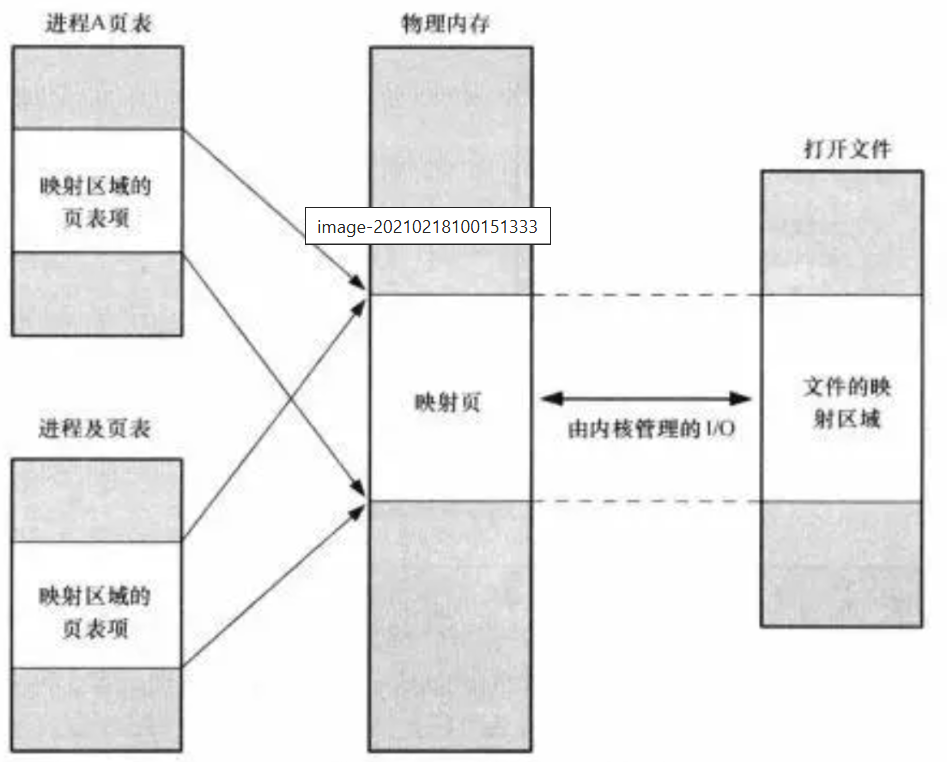
\includegraphics[width=0.5\textwidth]{two_proc_use_same}
	\caption{两个进程和一个文件在同一区域共享映射}
	\label{fig:two_proc_use_same}
\end{figure}

\subsubsection{VMA}

VMA (Virtual Memory Area)由一连串的虚拟地址组成,每个 VMA 都有相同的权限,指向相同的对象(文件、匿名内存等)

\subsection{实验过程}

\subsubsection{添加系统调用}

配置 \texttt{mmap} 和 \texttt{munmap} 的系统调用,如\cref{lst:add_mmap_and_munmap_syscall} 所示,并在 Makefile 中添加 \$U\_mmaptest\ 。

\begin{listing}[!htb]
	\begin{minted}{c}
// kernel.syscall.h
#define SYS_mmap   23
#define SYS_munmap 24

// kernel/syscall.c
extern uint64 sys_mmap(void);
extern uint64 sys_munmap(void);
...
[SYS_mmap]    sys_mmap,
[SYS_munmap]  sys_munmap,

// user/usys.pl
entry("mmap");
entry("munmap");

// user/user.h
void *mmap(void *, uint, int, int, int, uint);
int munmap(void *, int);
	\end{minted}
	\caption{配置 mmap 和 munmap 的系统调用}\label{lst:add_mmap_and_munmap_syscall}
\end{listing}

\subsubsection{实现 mmap 系统调用}

\begin{enumerate}
	\item 根据提示 3,定义 VMA 结构体,并添加到进程结构体中,如\cref{lst:VMA} 所示。
	\item 在 \texttt{allocproc} 中将 \texttt{vma} 数组初始化为全 0,如\cref{lst:memset_allocproc} 所示。
	\item 添                                                                                       加 mmap 系统调用的函数体。首先需要读取参数,之后在当前进程的 \texttt{vma} 
	字段中寻找一个空位,填充其对应的字段,就完成了记录该映射文件的工作,如\cref{lst:sys_mmap} 所示。
	\item 根据提示 5,此时访问对应的页面就会产生页面错误,需要在 \texttt{usertrap} 中进行处理,主要完成三项工作:分配物理页面,读取文件内容,添加映射关系,如\cref{lst:mmap_usertrap} 所示。
\end{enumerate}

\begin{listing}[!htb]
	\begin{minted}{c}
// kernel/param.h
#define NVMA 16

// kernel/proc.h
// 虚拟内存区域结构体
struct vm_area {
    int used;           // 是否已被使用
    uint64 addr;        // 起始地址
    int len;            // 长度
    int prot;           // 权限
    int flags;          // 标志位
    int vfd;            // 对应的文件描述符
    struct file* vfile; // 对应文件
    int offset;         // 文件偏移,本实验中一直为0
};

struct proc {
    ...
    struct vm_area vma[NVMA];    // 虚拟内存区域
}
	\end{minted}
	\caption{创建 vma 结构体并添加到 proc 中}\label{lst:VMA}
\end{listing}

\begin{listing}[!htb]
	\begin{minted}{c}
static struct proc*
allocproc(void)
{
    ...

    found:
    ...
    
    memset(&p->vma, 0, sizeof(p->vma));
    return p;
}
	\end{minted}
	\caption{在 allocproc 中初始化 vma 数组}\label{lst:memset_allocproc}
\end{listing}

\begin{listing}[!htb]
	\begin{minted}{c}
uint64
sys_mmap(void) {
    uint64 addr;
    int length;
    int prot;
    int flags;
    int vfd;
    struct file* vfile;
    int offset;
    uint64 err = 0xffffffffffffffff;

    // 获取系统调用参数
    if(argaddr(0, &addr) < 0 || argint(1, &length) < 0 || argint(2, &prot) < 0 || argint(3, &flags) < 0 || argfd(4, &vfd, &vfile) < 0 || argint(5,&offset) < 0)
        return err;

    // 实验提示中假定addr和offset为0,简化程序可能发生的情况
    if(addr != 0 || offset != 0 || length < 0)
        return err;

    // 文件不可写则不允许拥有PROT_WRITE权限时映射为MAP_SHARED
    if(vfile->writable == 0 && (prot & PROT_WRITE) != 0 && flags == MAP_SHARED)
        return err;
        
    struct proc* p = myproc();
    // 没有足够的虚拟地址空间
    if(p->sz + length > MAXVA)
        return err;

    // 遍历查找未使用的VMA结构体
    for(int i = 0; i < NVMA; ++i) {
        if(p->vma[i].used == 0) {
            p->vma[i].used = 1;
            p->vma[i].addr = p->sz;
            p->vma[i].len = length;
            p->vma[i].flags = flags;
            p->vma[i].prot = prot;
            p->vma[i].vfile = vfile;
            p->vma[i].vfd = vfd;
            p->vma[i].offset = offset;

            // 增加文件的引用计数
            filedup(vfile);

            p->sz += length;
            return p->vma[i].addr;
        }
    }
    return err;
}
	\end{minted}
	\caption{实现 sys\_mmap}\label{lst:sys_mmap}
\end{listing}

\begin{listing}[!htb]
	\begin{minted}{c}
void
usertrap(void)
{
    ...
    if(cause == 8) {
        ...
    } else if((which_dev = devintr()) != 0){
        // ok
    } else if(cause == 13 || cause == 15) {
        uint64 fault_va = r_stval();
        if(PGROUNDUP(p->trapframe->sp) - 1 < fault_va && fault_va < p->sz) {
            if(mmap_handler(r_stval(), cause) != 0) p->killed = 1;
        } 
        else
            p->killed = 1;
    } else {
        ...
    }
    ...
}

// 处理mmap惰性分配导致的页面错误
int mmap_handler(int va, int cause) {
    int i;
    struct proc* p = myproc();
    // 根据地址查找属于哪一个VMA
    for(i = 0; i < NVMA; ++i) 
        if(p->vma[i].used && p->vma[i].addr <= va && va <= p->vma[i].addr + p->vma[i].len - 1) 
            break;
    if(i == NVMA) return -1;
    
    int pte_flags = PTE_U;
    if(p->vma[i].prot & PROT_READ) pte_flags |= PTE_R;
    if(p->vma[i].prot & PROT_WRITE) pte_flags |= PTE_W;
    if(p->vma[i].prot & PROT_EXEC) pte_flags |= PTE_X;
    struct file* vf = p->vma[i].vfile;

    if(cause == 13 && vf->readable == 0) return -1;
    if(cause == 15 && vf->writable == 0) return -1;
    void* pa = kalloc();
    if(pa == 0) return -1;
    memset(pa, 0, PGSIZE);    
    // 读取文件内容
    ilock(vf->ip);
    int offset = p->vma[i].offset + PGROUNDDOWN(va - p->vma[i].addr);
    int readbytes = readi(vf->ip, 0, (uint64)pa, offset, PGSIZE);
    if(readbytes == 0) {
        iunlock(vf->ip);
        kfree(pa);
        return -1;
    }
    iunlock(vf->ip);
    // 添加页面映射
    if(mappages(p->pagetable, PGROUNDDOWN(va), PGSIZE, (uint64)pa, pte_flags) != 0) {
        kfree(pa);
        return -1;
    }
    return 0;
}
	\end{minted}
	\caption{在 usertrap 函数中处理缺页中断}\label{lst:mmap_usertrap}
\end{listing}

\subsubsection{实现 mmap 系统调用}

\begin{enumerate}
	\item 根据提示 6 实现 \texttt{munmap},且提示7中说明无需查看脏位就可写回,如\cref{lst:sys_munmap} 所示。
	\item 中断处理的懒加载方式允许了缺页错误的产生,因此在 \texttt{uvmcopy} 和
	\texttt{uvmunmap} 中需要删去对没有映射页面的报错,如\cref{lst:uvmcopy_and_uvmunmap} 所示。
\end{enumerate}

\begin{listing}[!htb]
	\begin{minted}{c}
uint64
sys_munmap(void) {
    uint64 addr;
    int length;
    if(argaddr(0, &addr) < 0 || argint(1, &length) < 0)
        return -1;

    int i;
    struct proc* p = myproc();
    for(i = 0; i < NVMA; ++i) {
        if(p->vma[i].used && p->vma[i].len >= length) {
            // 根据提示,munmap的地址范围只能是
            // 1. 起始位置
            if(p->vma[i].addr == addr) {
                p->vma[i].addr += length;
                p->vma[i].len -= length;
                break;
            }
            // 2. 结束位置
            if(addr + length == p->vma[i].addr + p->vma[i].len) {
                p->vma[i].len -= length;
                break;
            }
        }
    }
    if(i == NVMA)
        return -1;

    // 将MAP_SHARED页面写回文件系统
    if(p->vma[i].flags == MAP_SHARED && (p->vma[i].prot & PROT_WRITE) != 0) {
        filewrite(p->vma[i].vfile, addr, length);
    }

    // 判断此页面是否存在映射
    uvmunmap(p->pagetable, addr, length / PGSIZE, 1);
    
    // 当前VMA中全部映射都被取消
    if(p->vma[i].len == 0) {
        fileclose(p->vma[i].vfile);
        p->vma[i].used = 0;
    }

    return 0;
}
	\end{minted}
	\caption{实现 sys\_munmap}\label{lst:sys_munmap}
\end{listing}

\begin{listing}[!htb]
	\begin{minted}{c}
// kernel/vm.c
if((*pte & PTE_V) == 0)
    // panic("uvmunmap: not mapped");
    continue;

	\end{minted}
	\caption{在 uvmcopy 和 uvmunmap 中删去对没有映射页面的报错}\label{lst:uvmcopy_and_uvmunmap}
\end{listing}

\subsubsection{修改其他函数}

\begin{enumerate}
	\item 根据提示 8 修改 \texttt{exit},将进程的已映射区域取消映射,如\cref{lst:mmap_exit} 所示。
	\item 根据提示 9,修改 \texttt{fork},复制父进程的VMA并增加文件引用计数,如\cref{lst:mmap_fork} 所示。
\end{enumerate}

\begin{listing}[!htb]
	\begin{minted}{c}
void
exit(int status)
{
    // Close all open files.
    for(int fd = 0; fd < NOFILE; fd++){
        ...
    }

    // 将进程的已映射区域取消映射
    for(int i = 0; i < NVMA; ++i) {
        if(p->vma[i].used) {
            if(p->vma[i].flags == MAP_SHARED && (p->vma[i].prot & PROT_WRITE) != 0) {
                filewrite(p->vma[i].vfile, p->vma[i].addr, p->vma[i].len);
            }
            fileclose(p->vma[i].vfile);
            uvmunmap(p->pagetable, p->vma[i].addr, p->vma[i].len / PGSIZE, 1);
            p->vma[i].used = 0;
        }
    }

    begin_op();
    iput(p->cwd);
    end_op();
    ...
}	
	\end{minted}
	\caption{修改 exit 函数}\label{lst:mmap_exit}
\end{listing}

\begin{listing}[!htb]
	\begin{minted}{c}
int
fork(void)
{
    // increment reference counts on open file descriptors.
    for(i = 0; i < NOFILE; i++)
        ...
    ...
    
    // 复制父进程的VMA
    for(i = 0; i < NVMA; ++i) {
        if(p->vma[i].used) {
            memmove(&np->vma[i], &p->vma[i], sizeof(p->vma[i]));
            filedup(p->vma[i].vfile);
        }
    }
    
    safestrcpy(np->name, p->name, sizeof(p->name));
    ...
}
	\end{minted}
	\caption{修改 fork 函数}\label{lst:mmap_fork}
\end{listing}

\subsubsection{综合测试}

在 xv6-labs-2021 目录下创建一个 time.txt文件,记录该lab花费的时间。在 qemu 下使用 \texttt{mmaptest}、\texttt{usertests} 进行测试,在目录下使用 \texttt{make grade} 对 lab10 进行综合测试,测试通过,如\cref{fig:test_mmaptest}、\cref{fig:test_mmap_usertests}、\cref{fig:test_lab10} 所示。

\begin{figure}[!htb]
	\centering
	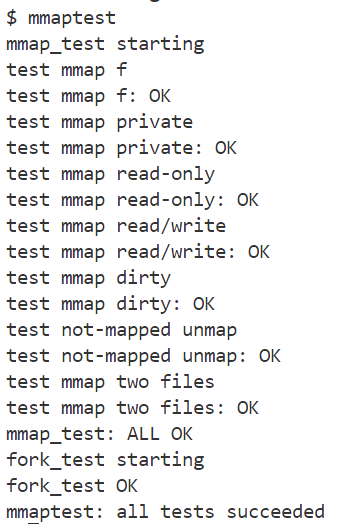
\includegraphics[width=0.4\textwidth]{test_mmaptest}
	\caption{测试 mmaptest}
	\label{fig:test_mmaptest}
\end{figure}

\begin{figure}[!htb]
	\centering
	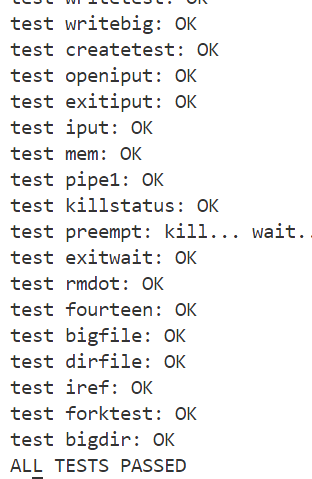
\includegraphics[width=0.4\textwidth]{test_mmap_usertests}
	\caption{测试 usertests}
	\label{fig:test_mmap_usertests}
\end{figure}

\begin{figure}[!htb]
	\centering
	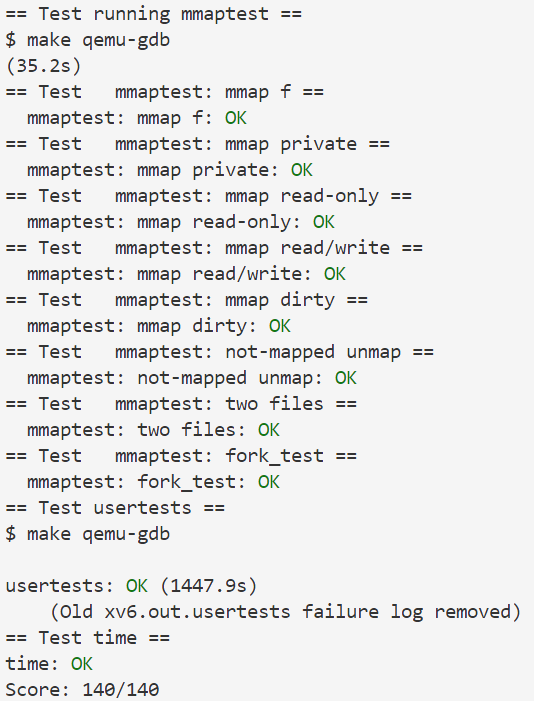
\includegraphics[width=0.45\textwidth]{test_lab10}
	\caption{测试 lab10}
	\label{fig:test_lab10}
\end{figure}

\subsection{实验小结}